\documentclass[border=1pt]{standalone}
\usepackage[dvipsnames]{xcolor}
\usepackage{tikz}                       % Graphen und kommutative Diagramme
\usetikzlibrary{patterns}               % Um schraffierte Formen in der tikzpicture-Umgebung zu zeichnen.


\begin{document}
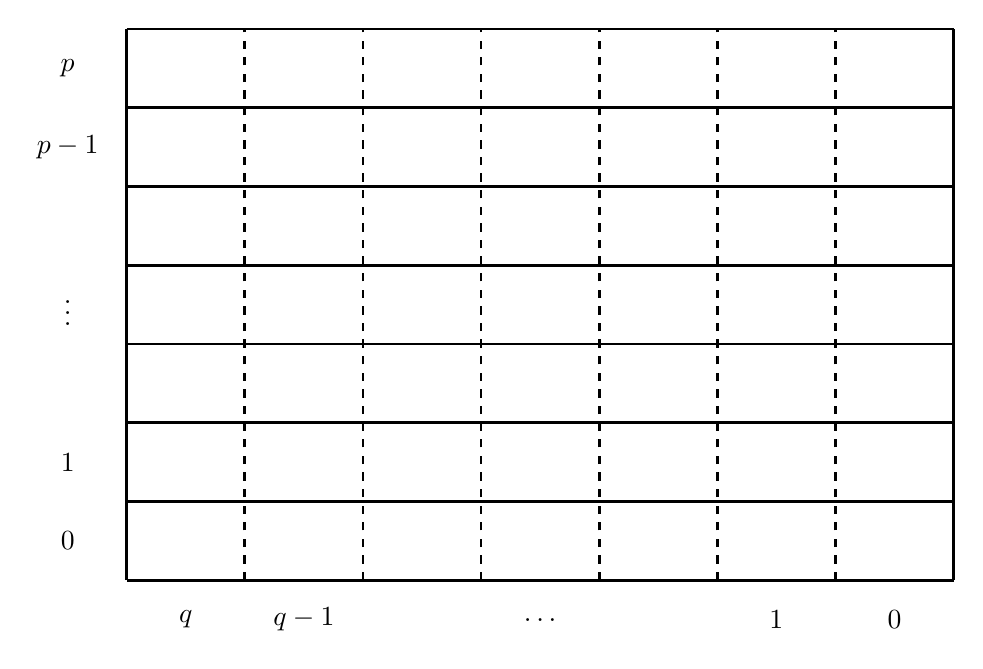
\begin{tikzpicture}[yscale=.8, xscale=1.2, x=1.25cm, y=1.25cm, line width=1pt]
    % Linien.
    \foreach \i in {0,...,7}
    {
        \draw[color=black] (0,\i) -- (7,\i);
    }
    \draw[color=black] (0,0) -- (0,7);
    \draw[color=black] (7,0) -- (7,7);
    \foreach \i in {1,...,6}
    {
        \draw[color=black, dashed] (\i,0) -- (\i,7);
    }
    
    % Beschriftung.
    \draw node at (-.5,6.5) {$p$};
    \draw node at (-.5,5.5) {$p-1$};
    \draw node at (-.5,3.5) {$\vdots$};
    \draw node at (-.5,1.5) {$1$};
    \draw node at (-.5,0.5) {$0$};
    
    \draw node at (0.5,-.5) {$q$};
    \draw node at (1.5,-.5) {$q-1$};
    \draw node at (3.5,-.5) {$\ldots$};
    \draw node at (5.5,-.5) {$1$};
    \draw node at (6.5,-.5) {$0$};
\end{tikzpicture}
\end{document}